\section{Trigonometric functions}\label{sec:trigonometric-functions}

\subsection{Conversion to radians (Page 173)}

\begin{multicols}{2}

    \begin{itemize}
        \item Given the angle $\theta$ in \underline{sexagecimal degrees} we can convert to radians as follows:
        \[
            \theta \times \dfrac{\pi}{180^\circ}
        \]
        \item Given the angle $\theta$ in \underline{radias} we can convert to sexagecimal degrees as follows:
        \[
            \theta \times \dfrac{180^\circ}{\pi}
        \]
    \end{itemize}

    \begin{figure}[H]
        \centering
        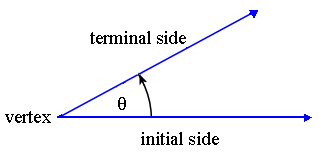
\includegraphics[width=6.5cm]{images/angle}
    \end{figure}

    \begin{figure}[H]
        \centering
        
\includegraphics[width=4cm]{images/img}
    \end{figure}
\end{multicols}



\subsection{Right triangle trigonometry (Page 179)}
Given the right triangle:

\begin{figure}[H]
    \centering
    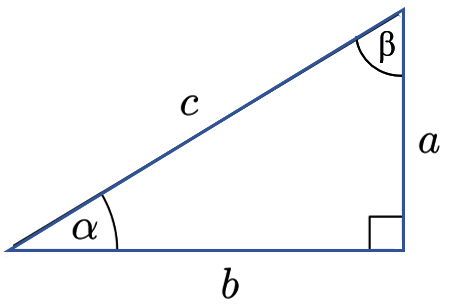
\includegraphics[width=5cm]{images/triangle}
\end{figure}
    \renewcommand{\arraystretch}{2.6}
    \begin{table}[H]
        \centering
        \begin{tabular}{|c|c|}
            \hline
            Basic trigonometric functions & Reciprocal trigonometric functions\\
            \hline \hline
            $\sin(A) = \dfrac{a}{c} = \dfrac{\text{leg opposite of }\angle A}{\text{hypotenuse}}$ & $\csc(A) = \dfrac{c}{a} = \dfrac{1}{\sin(A)}$ \\\hline
            $\cos(A) = \dfrac{b}{c} = \dfrac{\text{leg adjacent of }\angle A}{\text{hypotenuse}}$ & $\sec(A) = \dfrac{c}{b} = \dfrac{1}{\cos(A)}$ \\\hline
            $\tan(A) = \dfrac{a}{b} = \dfrac{\text{leg opposite of }\angle A}{\text{leg adjacent of }\angle A}$ & $\cot(A) = \dfrac{b}{a} = \dfrac{1}{\tan(A)}$ \\\hline
        \end{tabular}\label{tab:table}
    \end{table}



\subsection{Trigonometric functions of notable angles (Page 180)}

\begin{table}[H]
    \centering
    \begin{tabular}{|c|c|c|c|c|c|c|}
        \hline
        $\angle A$ & $\sin(A)$ & $\cos(A)$ & $\tan(A)$ & $\csc(A)$ & $\sec(A)$ & $\tan(A)$\\
        \hline \hline
        $30^\circ$ or $\dfrac{\pi}{6}$ & $\dfrac{1}{2}$ & $\dfrac{\sqrt{3}}{2}$ & $\dfrac{\sqrt{3}}{3}$ & 2 & $\dfrac{2\sqrt{3}}{3}$ & $\sqrt{3}$\\ \hline
        $45^\circ$ or $\dfrac{\pi}{4}$ & $\dfrac{\sqrt{2}}{2}$ & $\dfrac{\sqrt{2}}{2}$ & 1 & $\sqrt{2}$ & $\sqrt{2}$ & 1\\ \hline
        $60^\circ$ or $\dfrac{\pi}{3}$ & $\dfrac{\sqrt{3}}{2}$ & $\dfrac{1}{2}$ & $\sqrt{3}$ & $\dfrac{2\sqrt{3}}{3}$ & 2 & $\dfrac{\sqrt{3}}{3}$\\ \hline
    \end{tabular}\label{tab:table1}
\end{table}


\subsection{Inverse trigonometric functions (Page 182)}

\renewcommand{\arraystretch}{2.8}
\begin{table}[H]
    \centering
    \begin{tabular}{|c|p{4cm}|p{4cm}|p{4cm}|}
        \hline
        & Inverse Sine & Inverse Cosine & Inverse Tangent\\
        \hline
        Definition & If $\sin(\alpha) = x$, then $\sin^{-1}(x) = \alpha$. &  If $\cos(\alpha) = x$, then $\cos^{-1}(x) = \alpha$. &  If $\tan(\alpha) = x$, then $tan^{-1}(x) = \alpha$.\\\hline
        Example & If $\sin\left(\dfrac{\pi}{6}\right) = \dfrac{1}{2}$, then $\sin^{-1}\left(\dfrac{1}{2}\right) = \dfrac{\pi}{6}$. 
        & If $\cos\left(\dfrac{\pi}{6}\right) = \dfrac{\sqrt {3}}{2}$, then $\cos^{-1}\left(\dfrac{\sqrt {3}}{2}\right) = \dfrac{\pi}{6}$.
        & If $\tan\left(\dfrac{\pi}{6}\right) = \dfrac{\sqrt {3}}{3}$, then $\tan^{-1}\left(\dfrac{\sqrt {3}}{3}\right) = \dfrac{\pi}{6}$.\\\hline
    \end{tabular}\label{tab:table2}
\end{table}